\chapter{案例分析与实验评估}
\label{ch6}
在本小节,我们使用两个案例(智能温控系统\cite{David2012An}和机器人路径规划系统\cite{Lahijanian2010Motion})来展示本文提出的方法的有效性。首先,我们使用SysML建模语言对这两个案例进行建模,然后基于FMI标准,根据SysML建立的系统模型设计出协同仿真模型,接下来我们使用章节3提出的方法对系统协同仿真的可信性进行检测,之后将通过检测的协同仿真模型进行协同仿真并得到仿真迹,最后将得到仿真迹用章节4提出的方法进行验证分析并得到最终的验证分析结果。由于在章节3中我们已经使用了水箱案例的对系统协同仿真的可信性检测过程进行了详细的描述,这两个案例协同仿真的可信性检测过程与水箱案例类似。因此,在本章节我们不对这两个案例协同仿真的可信性检测的过程做过多的描述,而是重点关注:(1)这两个案例的模型针对特定的验证属性,通过统计模型检测算法验证之后得到的评估结果;(2)章节4提出的基于抽象和学习的统计模型检测算法的准确度及效率问题。
\section{案例一:智能温控系统}
智能温控系统在当今社会能源节约问题上起到十分重要的作用。该系统主要包含五个部分:\emph{房间温度、控制器、室外温度、加热器及用户}。控制器根据用户的行为及室内温度来控制加热器的开关,室内温度又受到室外温度、加热器及用户行为的影响。该系统的主要目的是评估某种控制策略下房间温度的舒适度及整个系统的能耗。
\subsection{系统建模与设计}

\subsection{系统验证分析}
本实验的分布式环境为五台处理器为英特尔(TM) i7-4790 (八核,主频3.6G赫兹)的计算机组成的集群。为了评估系统的行为和算法的性能,我们验证了以下三个验证属性,如表 \ref{tb:property}所示。
\begin{table}[t]
	\caption{智能温控系统的验证属性}
	\label{tb:property}
	\centering
	\begin{tabular}{c c c c}
		\hline
		序号 &  $(\delta,c)$ & 验证属性 & 验证结果 \\
		\hline
		$\phi_1$ & $(0.05,0.99)$  & $P_{=?}(F^{\leq48}~energy \geq 210)$ & 0.1778 \\ 
		$\phi_2$ & $(0.01,0.99)$  & $P_{=?}(F^{\leq48}~discomfort \geq 15)$ & 0.4861\\
		$\phi_3$ & $(0.02,0.9)$ & 
		\tabincell{c}{$P_{=?}(F^{\leq48}~ discomfort \leq 15$ \\ $\wedge~energy \geq 170)$} & 0.4535 \\
		\hline
	\end{tabular}
\end{table}
我们采用贝叶斯区间估计算法对上属三条验证属性进行评估分析并得到了验证结果。下面我们对表\ref{tb:property}的验证属性及验证结果进行分析:(1)$\phi_1$用来评估在48小时内能耗超过210的概率大小,我们得到的验证结果为0.1778,表示在48小时内系统能耗超过210的可能性比较小;(2)$\phi_1$用来评估48小时内,系统的不舒适度大于15的概率,得到的验证结果为0.4861;(3)$\phi_3$用来评估在48小时内,系统的不舒适度小于15且能耗大于170的概率,得到的验证结果为0.4535。由此,可以发现本文提出的方法可以有效的评估分析系统的行为。

\subsection{算法评估分析}
为了评估章节4提出的算法效率,在本小节我们针对以上的三个验证属性,从产生的迹的数量、验证所需要的时间及验证误差三个方面对比了多种统计模型检测算法:贝叶斯区间估计算法(BIE)、分布式的贝叶斯区间估计算法(DBIE)、基于抽象和学习的分布式统计模型检测算法(DAL-SMC)、经过优化的基于抽象和学习的分布式统计模型检测算法(DAL-SMC opt)、分布式的APMC\cite{herault2004approximate}算法(DAPMC),算法对比结果如图\ref{rs_sb}所示。
\begin{figure*}[htbp]
\centering{
		\subfigure[仿真迹的数量]{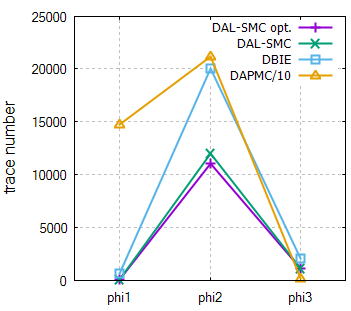
\includegraphics[width=1.5in,height=1.3in]{fig/4/sb-trace.png}
			\label{trace_sb}}
		\hfil
		\subfigure[验证时间]{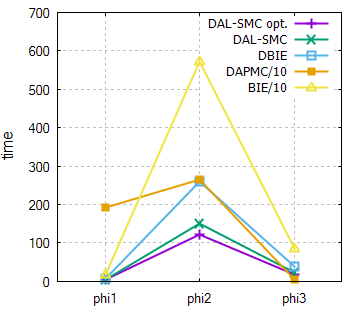
\includegraphics[width=1.5in,height=1.3in]{fig/4/sb-time.png}
			\label{time_sb}}
		\hfil
		\subfigure[验证误差]{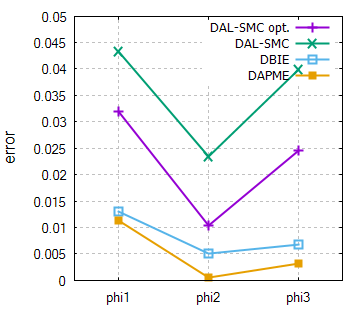
\includegraphics[width=1.5in,height=1.3in]{fig/4/sb-error.png}
			\label{error_sb}}
	\caption{智能温控系统案例算法对比}
	\label{rs_sb}
	}
\end{figure*}

图\ref{trace_sb}是算法产生的迹的数量对比,我们可以发现对于验证属性$\phi_2$,DAPMC消耗了大约200000条迹,然而DBIE只需要20000条迹即可以完成验证。 DAL-SMC和DAL-SMC opt.则需要更少量的迹(大约10000条)即可完成验证。 算法的验证时间的对比如图\ref{time_sb}所示,对于验证属性$\phi_2$,BIE需要6000秒,但分布式的BIE只需要大约250秒,DAL-SMC和DAL-SMC opt.需要更少的时间。图\ref{error_sb} 是算法的验证误差分析,对于验证属性$\phi1$,分布式BIE和DAPMC的误差大约为 0.013,DAL-SMC和DAL-SMC的验证误差大约为0.045和0.032。更详细的实验数据如表\ref{ta-rs}所示。 

\section{案例二:机器人路径规划系统}
在近些年来,机器人路径规划问题引起了学术界越来越多的人的关注。机器人路径规划问题的主要目标是要避免机器人与障碍物发生碰撞并最终能到达目的地。本案例在经典的机器人路径规划的基础上加上能耗,即机器人在移动过程中会消耗能量且在不同的时刻消耗的能量也可能存在区别。本案例主要包含机器人及障碍物两个部分,最终我们需要评估机器人产生的能耗及机器人发生碰撞的概率大小。
\subsection{系统建模与设计}

\subsection{系统验证分析}
\begin{table}[t]
	\caption{机器人路径规划的验证属性}
	\label{tb:robot}
	\centering
	\begin{tabular}{c c c c}
		\hline
		序号 & $(\delta,c)$ & 验证属性 & 验证结果 \\
		\hline
		$\phi_4$ & $(0.01,0.99)$ & $P_{=?}(F^{\leq100}~robot.collision)$ & 0.2675 \\ 
		$\phi_5$ & $(0.05,0.99)$ & $P_{=?}(F^{\leq100}~energy \geq 500)$ & 0.5211 \\
		$\phi_6$ & $(0.02,0.9)$ & 
		\tabincell{c}{$P_{=?}(F^{\leq100}~robot.collision$ \\ $\wedge~energy \geq 500)$} & 0.5296\\
		\hline
	\end{tabular}
\end{table}

我们采用贝叶斯区间估计算法对机器人路径规划的三条验证属性进行评估分析以得到验证结果。下面我们对表\ref{tb:robot}的验证属性及验证结果进行分析:(1)$\phi_4$用来评估在10小时内机器人与障碍物发生碰撞的概率大小,我们得到的验证结果为0.2675,表示在10小时内机器人与障碍物发生碰撞的可能性比较小;(2)$\phi_5$用来评估10小时内机器人消耗的能量大于500的概率大小,得到的验证结果为0.5211;(3)$\phi_6$用来评估在48小时内,10小时内机器人消耗的能量大于500的概率且不发生碰撞的概率大小,得到的验证结果为0.5296。由此,该案例也可有效说明本文提出的方法可以有效的评估分析系统的行为。

\subsection{算法评估分析}
通过用多种算法对机器人路径规划案例进行评估分析,得到的算法对比结果如图 \ref{rs_ro}所示:
\begin{figure*}[htbp]

\centering{
		\subfigure[仿真迹的数量]{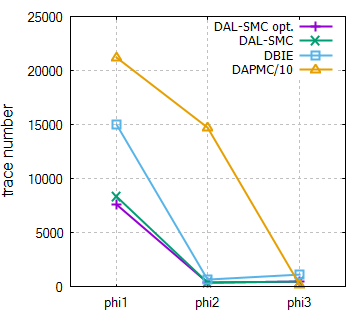
\includegraphics[width=1.5in,height=1.3in]{fig/4/ro-trace.png}
			\label{trace_ro}}
		\hfil
		\subfigure[验证时间]{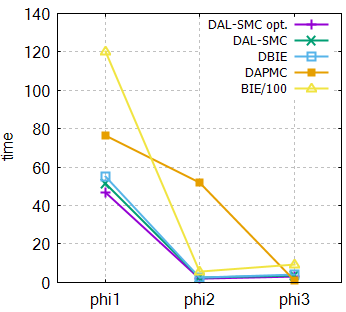
\includegraphics[width=1.5in,height=1.3in]{fig/4/ro-time.png}
			\label{time_ro}}
		\hfil
		\subfigure[验证误差]{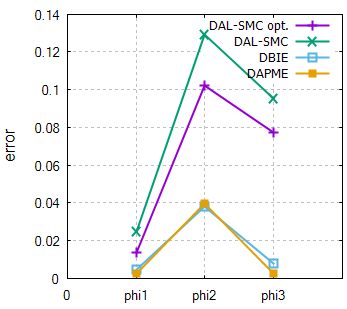
\includegraphics[width=1.5in,height=1.3in]{fig/4/ro-error.png}
			\label{error_ro}}
	\caption{机器人路径规划案例算法对比}
	\label{rs_ro}
	}
\end{figure*}

表\ref{ta-rs}给出了上述两个案例的算法对比的详细数据,下面我们针对验证属性 $\phi_2$来对算法的性能对比总结如下:
\begin{itemize}
\item
DAPMC的验证需要产生最多的仿真迹。相对于DAPMC,DBIE需要较少数量的迹即可以完成验证。此外,DAL-SMC相对于DBIE又将仿真迹的数量减少了大约一半。因此,针对产生仿真迹的数量来说,DAL-SMC是最高效的算法。
\item
对于验证而言,产生仿真迹的过程消耗了主要的验证时间。在分布式算法之中, DAPMC消耗时间最多,DAL-SMC得益于产生较少的仿真迹而相对DBIE消耗的时间较少 。在本实验中,我们使用40个核来实现分布式算法,我们发现经典BIE算法消耗的时间大约是分布式BIE算法的25倍,由此可以说明分布式技术在提高统计模型检测算法效率上是十分有效的。
\item
DAPMC和DBIE的验证误差较小,DAL-SMC的验证误差相对于DAPMC和DBIE较大一些。此外,我们发现DAL-SMC opt.的误差小于DAL-SMC的验证误差,说明我们提出的参数优化方法是有效的。
\end{itemize}
总的来说,DAL-SMC opt.算法得益于分布式技术和抽象与学习技术,在验证过程中需要产生最少的仿真迹和消耗最少的验证时间。此外,由于使用了章节4提出的参数优化方法,也使得将该算法的误差控制在了一个较小的范围之内。

\begin{table*}
\caption{实验结果}
\centering
\begin{tabular}{c c c c c c} 
        \hline  
        算法 & 验证属性 & 迹的数量 & 验证时间 & 验证误差\\
        \hline
        \multirow{6}{1.5cm}{DAPMC}  
                & $\phi1(0.05,0.99)$ &  147000&  1934.31&  0.0113\\ 
                & $\phi2(0.01,0.99)$ &  \textbf{211932} &  \textbf{2649.15} &  \textbf{0.0005}\\ 
                & $\phi3(0.02,0.9)$ &  1950&     38.05& 0.0032\\ 
                & $\phi4(0.01,0.99)$ &  211930&  76.282 &  0.0024\\ 
                & $\phi5(0.05,0.99)$ &  147550&  52.206&  0.0399\\ 
                & $\phi6(0.02,0.9)$ &  1850&     1.159& 0.0026\\     
        \hline 
        \multirow{6}{1.5cm}{DBIE}  
                & $\phi1(0.05,0.99)$ &  600&  7.895&  0.0131\\ 
                & $\phi2(0.01,0.99)$ &  \textbf{20000}&  \textbf{259.275} &  \textbf{0.0051} \\ 
                & $\phi3(0.02,0.9)$ &  2100& 38.057& 0.0068\\ 
                & $\phi4(0.01,0.99)$ & 15000&  55.281 &  0.0049\\ 
                & $\phi5(0.05,0.99)$ &  702&  2.483&  0.0382\\ 
                & $\phi6(0.02,0.9)$ &  1120& 4.226& 0.0078\\      
        \hline 
        \multirow{6}{1.5cm}{DAL-SMC}  
                & $\phi1(0.05,0.99)$ &  103&  5.685&  0.0433\\ 
                & $\phi2(0.01,0.99)$ &  \textbf{12000}&  \textbf{151.785} &  \textbf{0.0235} \\ 
                & $\phi3(0.02,0.9)$ &  1137& 22.841& 0.0399\\ 
                & $\phi4(0.01,0.99)$ &  8318&  41.68 &  0.0246\\ 
                & $\phi5(0.05,0.99)$ &  384&  2.32&  0.1295\\ 
                & $\phi6(0.02,0.9)$ &  520& 3.601& \ 0.0751\\      
        \hline 
         \multirow{6}{1.5cm}{DAL-SMC opt.}  
                & $\phi1(0.05,0.99)$ &  95.79&  4.65&  0.0319\\ 
                & $\phi2(0.01,0.99)$ &  \textbf{11040}&  \textbf{121.425} &  \textbf{0.0103}\\ 
                & $\phi3(0.02,0.9)$ &  1091& 18.73& 0.0246\\ 
                & $\phi4(0.01,0.99)$ &  7569&  36.512 &  0.0138\\ 
                & $\phi5(0.05,0.99)$ &  349&  1.81&  0.102\\ 
                & $\phi6(0.02,0.9)$ &  494& 3.171& 0.0575\\     
        \hline 
         \multirow{6}{1.5cm}{BIE}  
                & $\phi1(0.05,0.99)$ &  590&  175.44&  0.0121\\ 
                & $\phi2(0.01,0.99)$ &  \textbf{19586}&  \textbf{5730.67} &  \textbf{0.0047} \\ 
                & $\phi3(0.02,0.9)$ &  2040& 845.73& 0.0063\\ 
                & $\phi4(0.01,0.99)$ & 15400&  1202.467 &  0.0044\\ 
                & $\phi5(0.05,0.99)$ &  762&  55.221&  0.0352\\ 
                & $\phi6(0.02,0.9)$ &  1150& 91.98& 0.0069\\      
        \hline 
\end{tabular} 
\label{ta-rs}
\end{table*}

\section{本章小结}
本文使用两个案例来说明本文提出方法的可行性,首先对案例进行了建模和设计,然后重点在系统的验证分析小节中展示了本方法在对系统进行评估分析时的有效性,并在算法评估分析小节结合两个案例,从多个方面对比了多种算法的性能,从而展示了我们本文提出的基于抽象和学习的分布式统计模型检测算法的高效性和准确性。
